\section{Optimizers}

\begin{itemize}
	\item SGD (Stochastic Gradient Descent)
	\item Batch Gradient Descent
	\item Mini Batch Gradient Descent
	\item RMSprop (Root Mean Square Propagation)
	\item Adam (Adaptive Moment Estimation)
	\item AdamW
	\item Adadelta
	\item Adagrad
	\item Adafactor
	\item Adamax
	\item FTRL (Follow-The-Regularized-Leader)
	\item Lion (Layer-wise Adaptive Inertia Optimizer)
	\item Nadam (Nesterov-accelerated Adaptive Moment Estimation)
	\item Loss Scaling
	\item Sparse Adam
	\item L-BFGS (Limited-memory Broyden-Fletcher-Goldfarb-Shanno)
	\item RAdam (Rectified Adam)
	\item Averaged Stochastic Gradient Descent (Averaged SGD)
	\item Rprop (Resilient Propagation)
\end{itemize}

\newpage

\subsection{SGD (Stochastic Gradient Descent)}
Gradyan azalmada tüm veri seti kullanılırken stokastik gradyan azalmada tek bir örneklem kullanılır. Her bir adımda bir örnek seçer ve bu örneğe göre gradyanı hesaplar. Bu yüzden "stokastik" olarak adlandırılır. Küçük veri kümelerinde kullanışlıdır. Tek örnek ile işlem yapıldığı için global minimuma doğru kararlı bir şekilde ilerleme görülmez. Minimaya ulaşmak için daha fazla iterasyon sayısına ihtiyaç duyar. Her iterasyonda rastgele bir veri örneği kullandığı için, gradyan tahminleri çok değişken olabilir ve bu da öğrenme sürecinde gürültüye neden olabilir. ürültü nedeniyle, SGD'nin yakınsama süreci kararsız olabilir ve minimuma ulaşmada zorluk yaşanabilir.

\begin{figure}[h]
    \centering
    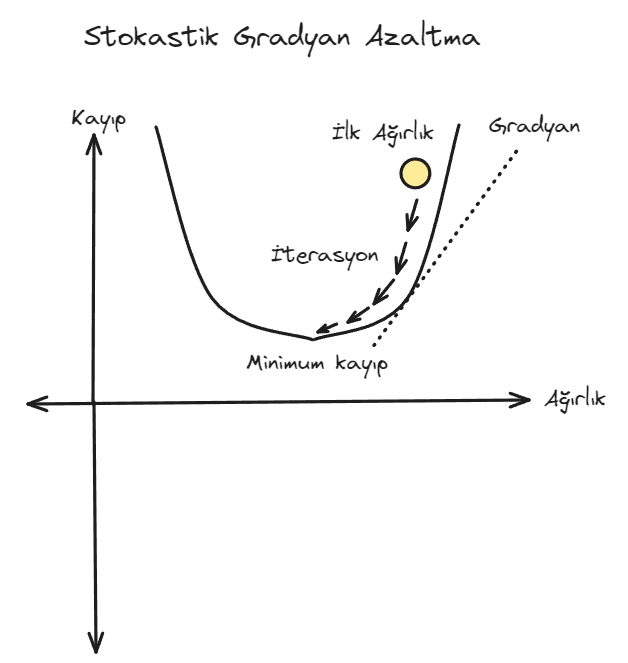
\includegraphics[width=0.5\textwidth]{images/sgd_optimizer.png}
    \caption{SGD optimizasyon algoritması.}
    \label{fig:enter-label}
\end{figure}


\[\theta_{t+1} = \theta_{t} - \alpha \nabla f(\theta_{t})\]

\begin{itemize}
	\item $\theta_(t)$: t zamandaki parametre vektörü
	\item $\alpha$: öğrenme oranı,
	\item $\nabla f(\theta_{t})$: fonksiyonun t zamanındaki gradyanı.
\end{itemize}

\subsubsection{Çalışma Adımları}

Elimizde $L(\theta) = (\theta - 4)^2$ gibi bir kayıp fonksiyonu olsun. Buradaki $\theta = 0.0$ başlangıç değerine sahip olsun.  Öğrenme oranı $\alpha = 0.1$ olsun. Kayıp fonksiyonunu $\theta$ açısından türevini alarak gradyanı hesaplayalım.

\[ g(\theta) = \frac{d}{d \theta} (\theta - 4)^2 = 2 (\theta - 4) \]

Başlangıç parametresi $\theta_0 = 0$ olduğundan:

\[ g_0 = 2 (0 - 4) = -8 \]

SGD formülünü kullanarak parametreler güncellenir.

\[ \theta_1 = \theta_0 - \eta \cdot g_0 \]

\[ \theta_1 = 0 - 0.1 \cdot (-8) = 0.8 \]

Bu işlemler belirli bir iterasyon boyunda tekrarlanır.

\subsubsection{Python Kodu}

\begin{lstlisting}[language=Python]
import numpy as np

class SGD:
    def __init__(self, learning_rate=0.01, num_iterations=1000):
        self.learning_rate = learning_rate
        self.num_iterations = num_iterations

    def loss_function(self, X, y):
        return np.mean((X.dot(self.theta) - y) ** 2)

    def grad(self, X, y):
        return 2 / len(X) * X.T.dot(X.dot(self.theta) - y)
    
    def fit(self, X, y):
        X = np.c_[np.ones((X.shape[0], 1)), X]

        self.theta = np.zeros(X.shape[1])

        for iteration in range(self.num_iterations):
            gradients = self.grad(X, y)

            self.theta -= self.learning_rate * gradients

            if iteration % 100 == 0:
                loss = self.loss_function(X, y)

    def predict(self, X):
        X = np.c_[np.ones((X.shape[0], 1)), X]
        return X.dot(self.theta)
\end{lstlisting}

\newpage

\subsection{Batch Gradient Descent}

Tüm eğitim örneklerini bir arada kullanarak her bir iterasyonda gradyanı hesaplayar ve parametreleri günceller. Veri setinin tamamını kullanarak güncellemeler yapmak daha kararlı ve doğru sonuçlar elde etmeyi sağlar fakat büyük veri setleri için hesaplama maliyeti yüksek olabilir. Tüm veri seti kullanılarak tek bir gradyan hesaplanır. Parametreler, tüm veri setinin gradyanı hesaplandıktan sonra bir kez güncellenir.

\[\theta = \theta - \alpha \nabla J(\theta)\]

\begin{itemize}
	\item $\theta$: optimize edilen parametrelerin vektörü,
	\item $\alpha$: öğrenme oranı,
	\item $J(\theta)$: maliyet fonksiyonunun gradyanı.
\end{itemize}

\subsubsection{Çalışma Adımları}

Örnek kayıp fonksiyonu:

\[ L(\theta) = \frac{1}{m} \sum_{i=1}^{m} (\theta x^{(i)} - y^{(i)})^2 \]

Başlangıç parametresi $\theta_0 = 0$, öğrenme oranı $\eta = 0.1$, $X = [1, 2, 3]$ ve $y = [2, 4, 6]$ olsun. Bu, $y = 2x$ doğrusal ilişkisinin basit bir modelidir.

Gradyan hesaplaması için önce her bir verideki tahmini bulunur ve farkları toplanır. Parametrelerin ilk değeri $\theta_0 = 0$ iken, tahmin edilen değerler:

\[ \hat{y}^{(i)} = \theta_0 \cdot x^{(i)} \]

\[ \hat{y}^{(1)} = 0 \cdot 1 = 0 \]

\[ \hat{y}^{(2)} = 0 \cdot 1 = 0 \]

\[ \hat{y}^{(3)} = 0 \cdot 1 = 0 \]

Kayıp fonksiyonunun $\theta$'ya göre türevini alalım:

\[ \frac{\partial}{\partial \theta} J(\theta) = \frac{2}{m} \sum_{i=1}^{m} x^{(i)} (\theta x^{(i)} - y^{(i)}) \]

Bu örnekte m = 3, böylece:

\[ g_0 = \frac{2}{3} [1(0 \cdot 1 - 2) + 2(0 \cdot 2 - 4) + 3(0 \cdot 3 - 6)] \]
\[ g_0 = \frac{2}{3} [- 2 - 8 - 18] = \frac{2}{3} \cdot (-28) = -18.67 \]

Batch Gradient Descent formülü ile parametreler güncellenir.

\[ \theta_{t+1} = \theta_t - \eta \cdot g_t \]

\[ \theta_1 = \theta_0 - \eta \cdot g_0 \]

\[ \theta_1 = 0 - 0.1 \cdot (-18.67) = 1.867 \]

Aynı işlemler tekrarlanarak $\theta_2$ bulunur.

\subsubsection{Python Kodu}

\begin{lstlisting}[language=Python]
class BatchGradientDescent:
    def __init__(self, learning_rate=0.01, num_iterations=1000):
        self.learning_rate = learning_rate
        self.num_iterations = num_iterations

    def loss_function(self, X, y):
        return np.mean((X.dot(self.theta) - y) ** 2)

    def grad(self, X, y):
        return 2 / len(X) * X.T.dot(X.dot(self.theta) - y)
    
    def fit(self, X, y):
        X = np.c_[np.ones((X.shape[0], 1)), X]

        self.theta = np.zeros(X.shape[1])

        for iteration in range(self.num_iterations):
            gradients = self.grad(X, y)

            self.theta -= self.learning_rate * gradients

            if iteration % 100 == 0:
                loss = self.loss_function(X, y)

    def predict(self, X):
        X = np.c_[np.ones((X.shape[0], 1)), X]
        return X.dot(self.theta)
\end{lstlisting}

\newpage

\subsection{Mini Batch Gradient Descent}

Her bir iterasyonda tüm veri setini değil, belirli bir alt küme (mini batch) üzerinde işlem yapar. Bu, batch gradient descent'in hesaplama maliyetini azaltır ve stochastic gradient descent'in rastgele dalgalanmaları azaltmasını sağlar. Mini batch içerisindeki örnekler için gradyanlar hesaplanır. Belirli bir mini batch üzerinde gradyan hesaplandığı için güncelleme sıklığı batch gradient descent'e göre daha sık, stochastic gradient descent'e göre daha düzenlidir.

\[\theta = \theta - \alpha \cdot \frac{1}{|\text{mini batch}|} \sum_{i=1}^{|\text{mini batch}|} \nabla J(\theta;x^{(i)},y^{(i)})\]

\begin{itemize}
	\item $\theta$: optimize edilen parametrelerin vektörü,
	\item $\alpha$: öğrenme oranı,
	\item ${|\text{mini batch}|}$: mini batch'deki örneklerin sayısı,
	\item $J(\theta;x^{(i)},y^{(i)})$: maliyet fonksiyonu,
	\item $x^{i}$ ve $y^{i}$: eğitim veri setindeki i'inci örnek.
\end{itemize}

\subsubsection{Çalışma Adımları}

Örnek kayıp fonksiyonu:

\[ L(\theta) = \frac{1}{m} \sum_{i=1}^{m} (\theta x^{(i)} - y^{(i)})^2 \]

Başlangıç parametresi $\theta_0 = 0$, öğrenme oranı $\eta = 0.1$, mini-batch boyutu $B$ = 2, $X = [1, 2, 3]$ ve $y = [2, 4, 6]$ olsun. Bu, $y = 2x$ doğrusal ilişkisinin basit bir modelidir.

Mini-batch boyutu 2 olduğunda göre, $X = [1, 2]$ ve $y = [2, 4]$ kullanarak mini-batch seçimi yapılır. 

Gradyan hesaplaması için önce her bir verideki tahmini bulunur ve farkları toplanır. Parametrelerin ilk değeri $\theta_0 = 0$ iken, tahmin edilen değerler:

\[ \hat{y}^{(i)} = \theta_0 \cdot x^{(i)} \]

\[ \hat{y}^{(1)} = 0 \cdot 1 = 0 \]

\[ \hat{y}^{(2)} = 0 \cdot 1 = 0 \]

Kayıp fonksiyonunun $\theta$'ya göre türevini alalım:

\[ g_0 = \frac{2}{B} \sum_{i=1}^{2} (\theta x^{(i)} - y^{(i)})^2 \]

\[ g_0 = \frac{2}{2} [1(0 \cdot 1 - 2) + 2(0 \cdot 2 - 4)]\]

\[ g_0 = 1 [- 2 - 8] = -10 \]

Mini-batch Gradient Descent formülünü kullanarak parametre güncellemesi yapılır.

\[ \theta_1 = \theta_0 - \eta \cdot g_0 \]

\[ \theta_1 = 0 - 0.a \cdot (-10) = 1 \]

İkinci mini batch için $X = [3]$ ve $y = [6]$ seçilir. $\theta_1 = 1$ gradyan hesaplanır.

\[ \hat{y}^{(3)} = 1 \cdot 3 = 3 \]

\[ g_1 = \frac{2}{1} \cdot 3 (1 \cdot 3 - 6) = 6 \cdot (-3) = -18 \]

\[ \theta_2 = 1 - 0.1 \cdot (-18) = 2.8 \]

Bu işlemi tüm mini-batch'ler için tekrarlayarak parametre güncellemelerine devam edilir.

\subsubsection{Python Kodu}

\begin{lstlisting}[language=Python]
class MiniBatchGradientDescent:
    def __init__(self, learning_rate=0.01, num_iterations=100, batch_size=32):
        self.learning_rate = learning_rate
        self.num_iterations = num_iterations
        self.batch_size = batch_size

    def loss_function(self, X, y):
        return np.mean((X.dot(self.theta) - y) ** 2)
        
    def grad(self, X, y):
        return 2 / len(X) * X.T.dot(X.dot(self.theta) - y)
    
    def fit(self, X, y):
        X = np.c_[np.ones((X.shape[0], 1)), X]

        self.theta = np.zeros(X.shape[1])
        
        for iteration in range(1, self.num_iterations + 1):
            indices = np.random.permutation(len(X))
            X_shuffled = X[indices]
            y_shuffled = y[indices]

            for i in range(0, len(X), self.batch_size):
                X_batch = X_shuffled[i:i + self.batch_size]
                y_batch = y_shuffled[i:i + self.batch_size]

                gradients = self.grad(X, y)
                self.theta -= self.learning_rate * gradients

            if iteration % 100 == 0:
                loss = self.loss_function(X, y)

    def predict(self, X):
        X = np.c_[np.ones((X.shape[0], 1)), X]
        return X.dot(self.theta)
\end{lstlisting}

\newpage

\subsection{RMSprop (Root Mean Square Propagation)}
Gradyanlara bağlı olarak öğrenme oranını (learning rate) ayarlar. Her parametreyi ayrı ayrı günceller. Eğer bir boyutta gradyanlar büyük ise RMSprop tarafından hesaplanan güncelleme oranı düşer; küçük ise güncelleme oranı artar. Daha az varyans gösteren parametreler daha fazla güncellenir; daha fazla varyans gösteren parametreler daha az güncellenir. Büyük veri setlerinde iyi çalışır. Bu algoritma, AdaGrad algoritmasına benzer, ancak AdaGrad'ın zamanla küçülen öğrenme oranı problemine çözüm getirir. RMSprop, karelenmiş gradyanların ortalamasını tutar ve her bir ağırlık için öğrenme oranını bu ortalama üzerinden ölçeklendirir.

\begin{figure}[h]
    \centering
    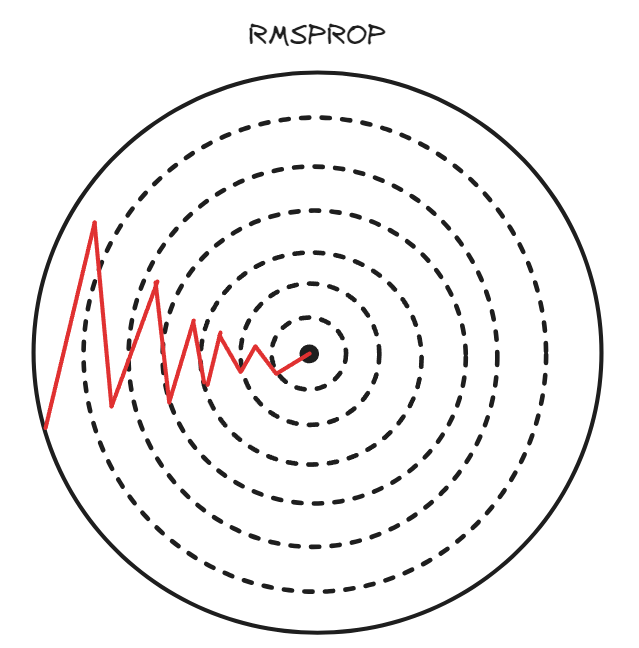
\includegraphics[width=0.5\textwidth]{images/rmsprop_optimizer.png}
    \caption{RMSprop optimizasyon algoritması.}
    \label{fig:enter-label}
\end{figure}

\begin{align*}
E[g^2]_t & = \rho E[g^2]_{t-1} + (1 - \rho) (\nabla f(\theta_t))^2 \\
\theta_{t+1} & = \theta_t - \frac{\alpha}{\sqrt{E[g^2]_t + \epsilon}} \nabla f(\theta_t)
\end{align*}

\begin{itemize}
	\item $\theta_(t)$: t zamanındaki parametre vektörü,
	\item $\nabla f(\theta_{t})$: fonksiyonun t zamanıdaki gradyanı,
	\item $E[g^2]_t$: gradyanların karesinin üstel hareketli ortalaması,
	\item $\rho$: gradyan karesinin üstel azaltma oranı,
	\item $\alpha$: öğrenme oranı,
	\item $\epsilon$: düzeltme terimi.
\end{itemize}

\subsubsection{Çalışma Adımları}

Örnek kayıp fonksiyonu:

\[ L(\theta) = \frac{1}{m} \sum_{i=1}^{m} (\theta x^{(i)} - y^{(i)})^2 \]

Başlangıç parametresi $\theta_0 = 0$, öğrenme oranı $\eta = 0.1$, $\gamma = 0.9$, $X = [1, 2]$ ve $y = [2, 4]$ olsun. Bu, $y = 2x$ doğrusal ilişkisinin basit bir modelidir.

\[ \nabla_\theta J(\theta_0) = \frac{1}{2} [1(0 \cdot 1 - 2) + 2(0 \cdot 2 - 4)] = -10 \]

Gradyanın karesi:

\[ \nabla_\theta J(\theta_0)^2 = (-10)^2 = 100 \]

RMSprop formülünü kullanarak gradyan karelerinin üstel hareketli ortalamasını hesaplanır:

\[ S_t = \gamma S_{t-1} + (1 - \gamma) \nabla_\theta J(\theta_t)^2 \]

Başlangıçta $S_0 = 0$ böylece:

\[ S_1 = 0.9 \cdot 0 + 0.1 \cdot 100 = 10 \]

Gradyanın karelerinin ortalaması kullanılarak parametre güncellemesi yapılır:

\[ \theta_{t+1} = \theta_t - \frac{\eta}{\sqrt{S_t} + \epsilon} \nabla_\theta J(\theta_t) \]

\[ \theta_1 = 0 - \frac{0.1}{\sqrt{10 + \epsilon}} (-10) = 0.316 \]

$\theta_1 = 0.316$ ile yeni gradyanı ve karelerini hesaplanır:

\[ \nabla_\theta J(\theta_1) \approx -7.37 \]

Gradyanın karesi:

\[ \nabla_\theta J(\theta_1)^2 \approx 54.37 \]

Gradyan karelerinin üstel hareketli ortalaması:

\[ S_2 = 0.9 \cdot 10 + 0.1 \cdot 54.37 = 14.43 \]

Parametre güncellemesi:

\[ \theta_2 = 0.316 - \frac{0.1}{\sqrt{14.43 + \epsilon} (-7.37)} = 0.509 \]

Bu adımları veri boyunca tekrarlayarak, parametre güncellemeleri yapılır ve model optimize edilir.

\subsubsection{Python Kodu}

\begin{lstlisting}[language=Python]
class RMSprop:
    def __init__(self, learning_rate=0.01, rho=0.9, epsilon=1e-8, num_iterations=1000):
        self.learning_rate = learning_rate
        self.rho = rho
        self.epsilon = epsilon
        self.num_iterations = num_iterations

    def loss_function(self, X, y):
        m = len(y)
        predictions = self.theta * X
        return (1 / m) * np.sum((predictions - y) ** 2)

    def grad(self, X, y):
        return 2 / len(X) * X.T.dot(X.dot(self.theta) - y)
    
    def fit(self, X, y):
        X = np.c_[np.ones((X.shape[0], 1)), X]

        self.theta = np.zeros(X.shape[1])

        Eg2 = np.zeros(X.shape[1])

        for iteration in range(1, self.num_iterations + 1):
            gradients = self.grad(X, y)

            Eg2 = self.rho * Eg2 + (1 - self.rho) * gradients ** 2

            self.theta -= self.learning_rate / (np.sqrt(Eg2) + self.epsilon) * gradients

            if iteration % 100 == 0:
                loss = self.loss_function(X, y)

    def predict(self, X):
        X = np.c_[np.ones((X.shape[0], 1)), X]
        return X.dot(self.theta)
\end{lstlisting}

\newpage

\subsection{Adam (Adaptive Moment Estimation)}
Momentum ve RMSprop yöntemlerinin birleşimidir. Birinci ve ikinci momentlerin (hareketli ortalama) eksponensiyel bir şekilde azalan ortalama değerlerini korur ve bu sayede gradyanları güvenilir bir şekilde tahmin eder. Gürültülü veri setleri için uygundur.

\begin{align*}
m_{t+1} & = \beta_{1}m_{t} + (1 - \beta_{1})\nabla f(\theta_{t}) \\
v_{t+1} & = \beta_{2}v_{t} + (1 - \beta_{2})(\nabla f(\theta_{t}))^2 \\
\hat{m}_{t+1} & = \frac{m_{t+1}}{1 - \beta_{1}^{t+1}} \\
\hat{v}_{t+1} & = \frac{v_{t+1}}{1 - \beta_{2}^{t+1}} \\
\theta_{t+1} & = \theta_{t} - \frac{\alpha}{\sqrt{\hat{v}_{t+1}} + \epsilon} \hat{m}_{t+1}
\end{align*}

\begin{itemize}
	\item $\theta_(t)$: t zamanındaki parametre vektörü,
	\item $\nabla f(\theta_{t})$: fonksiyonun t zamanıdaki gradyanı,
	\item $m_{t}$ ve $v_(t)$: t zamanıdaki birinci ve ikinci moment tahminleri,
	\item $\beta_{1}$ ve $\beta_{2}$: momentlerin üstel azalma oranları,
	\item $\hat{m}_{t+1}$ ve $\hat{v}_{t+1}$: düzeltmiş moment tahminleri,
	\item $\alpha$: öğrenme oranı,
	\item $\epsilon$: düzeltme terimi.
\end{itemize}

\subsubsection{Çalışma Adımları}

Örnek kayıp fonksiyonu:

\[ L(\theta) = \frac{1}{m} \sum_{i=1}^{m} (\theta x^{(i)} - y^{(i)})^2 \]

Başlangıç parametresi $\theta_0 = 0$, öğrenme oranı $\eta = 0.1$, $\beta_1 = 0.9$, $\beta_2 = 0.999$, $X = [1, 2]$ ve $y = [2, 4]$ olsun. Bu, $y = 2x$ doğrusal ilişkisinin basit bir modelidir.

\[ \nabla_\theta J(\theta_0) = \frac{1}{2} [1(0 \cdot 1 - 2) + 2(0 \cdot 2 - 4)] = -10 \]

Birinci moment $m_0 = 0$ ve ikinci moment $v_0 = 0$ ile başlanır. Birinci moment:

\[ m_t = \beta_1 m_{t-1} + (1 - \beta_1) \nabla_\theta J(\theta_t) \]

\[ m_1 = 0.9 \cdot 0 + 0.1 \cdot (-10) = -1 \]

İkinci moment:

\[ v_t = \beta_2 v_{t-1} + (1 - \beta_2) \nabla_\theta J(\theta_t)^2 \]

\[ v_1 = 0.999 \cdot 0 + 0.001 \cdot 100 = 0.1 \]

Birinci moment bias düzeltmesi:

\[ \hat{m}_t = \frac{m_t}{1 - \beta_{1}^t} \]

\[ \hat{m}_1 = \frac{-1}{1 - 0.9} = -10 \]

İkinci moment bias düzeltmesi:

\[ \hat{v}_t = \frac{v_t}{1 - \beta_{2}^t} \]

\[ \hat{v}_1 = \frac{0.1}{1 - 0.999} = 100 \]

Parametre güncelleme

\[ \theta_{t+1} = \theta_t - \frac{\eta}{\sqrt{\hat{v}_t} + \epsilon} \hat{m}_t \]

\[ \theta_{1} = 0 - \frac{0.1}{\sqrt{100} + \epsilon} (-10) = 0.1 \]

\subsubsection{Python Kodu}

\begin{lstlisting}[language=Python]
class Adam:
    def __init__(self,
                 learning_rate=0.001,
                 beta1=0.9,
                 beta2=0.999,
                 epsilon=1e-8,
                 num_iterations=1000):

        self.learning_rate = learning_rate
        self.beta1 = beta1
        self.beta2 = beta2
        self.epsilon = epsilon
        self.num_iterations = num_iterations

    def loss_function(self, X, y):
        m = len(y)
        predictions = self.theta * X
        return (1 / m) * np.sum((predictions - y) ** 2)
        
    def grad(self, X, y):
        return 2 / len(X) * X.T.dot(X.dot(self.theta) - y)

    def fit(self, X, y):
        X = np.c_[np.ones((X.shape[0], 1)), X]

        self.theta = np.zeros(X.shape[1])
        
        m = np.zeros(X.shape[1])
        v = np.zeros(X.shape[1])

        for iteration in range(1, self.num_iterations + 1):
            gradients = self.grad(X, y)

            m = self.beta1 * m + (1 - self.beta1) * gradients
            v = self.beta2 * v + (1 - self.beta2) * gradients ** 2

            m_hat = m / (1 - self.beta1 ** iteration)
            v_hat = v / (1 - self.beta2 ** iteration)

            self.theta -= self.learning_rate * m_hat / (np.sqrt(v_hat) + self.epsilon)

            if iteration % 100 == 0:
                loss = self.loss_function(X, y)

    def predict(self, X):
        X = np.c_[np.ones((X.shape[0], 1)), X]
        return X.dot(self.theta)
\end{lstlisting}

\newpage

\subsection{AdamW}
Adam yöntemine ağırlık çarpımı (weight decay) eklenmiş bir versiyonudur. Ağırlık çarpımı, modelin karmaşıklığını kontrol etmek ve aşırı uydurmaya karşı koymak için kullanılan bir tekniktir.

\begin{align*}
m_{t+1} & = \beta_{1}m_{t} + (1 - \beta_{1})\nabla f(\theta_{t}) \\
v_{t+1} & = \beta_{2}v_{t} + (1 - \beta_{2})(\nabla f(\theta_{t}))^2 \\
\hat{m}_{t+1} & = \frac{m_{t+1}}{1 - \beta_{1}^{t+1}} \\
\hat{v}_{t+1} & = \frac{v_{t+1}}{1 - \beta_{2}^{t+1}} \\
\theta_{t+1} & = \theta_{t} - \frac{\alpha}{\sqrt{\hat{v}_{t+1}} + \epsilon} \hat{m}_{t+1} - \lambda \theta_{t}
\end{align*}

\begin{itemize}
	\item $\theta_(t)$: t zamanındaki parametre vektörü,
	\item $\nabla f(\theta_{t})$: fonksiyonun t zamanıdaki gradyanı,
	\item $m_{t}$ ve $v_(t)$: t zamanıdaki birinci ve ikinci moment tahminleri,
	\item $\beta_{1}$ ve $\beta_{2}$: momentlerin üstel azalma oranları,
	\item $\hat{m}_{t+1}$ ve $\hat{v}_{t+1}$: düzeltmiş moment tahminleri,
	\item $\alpha$: öğrenme oranı,
	\item $\epsilon$: düzeltme terimi,
	\item $\lambda$: ağırlık bozulma (weight decay) parametresi.
\end{itemize}

\subsubsection{Çalışma Adımları}

Örnek kayıp fonksiyonu:

\[ L(\theta) = \frac{1}{m} \sum_{i=1}^{m} (\theta x^{(i)} - y^{(i)})^2 \]

Başlangıç parametresi $\theta_0 = 0$, öğrenme oranı $\eta = 0.1$, $\beta_1 = 0.9$, $\beta_2 = 0.999$, $\alpha = 0.01$,  $X = [1, 2]$ ve $y = [2, 4]$ olsun. Bu, $y = 2x$ doğrusal ilişkisinin basit bir modelidir.

\[ \nabla_\theta J(\theta_0) = \frac{1}{2} [1(0 \cdot 1 - 2) + 2(0 \cdot 2 - 4)] = -10 \]

Birinci moment $m_0 = 0$ ve ikinci moment $v_0 = 0$ ile başlanır. Birinci moment:

\[ m_t = \beta_1 m_{t-1} + (1 - \beta_1) \nabla_\theta J(\theta_t) \]

\[ m_1 = 0.9 \cdot 0 + 0.1 \cdot (-10) = -1 \]

İkinci moment:

\[ v_t = \beta_2 v_{t-1} + (1 - \beta_2) \nabla_\theta J(\theta_t)^2 \]

\[ v_1 = 0.999 \cdot 0 + 0.001 \cdot 100 = 0.1 \]

Birinci moment bias düzeltmesi:

\[ \hat{m}_t = \frac{m_t}{1 - \beta_{1}^t} \]

\[ \hat{m}_1 = \frac{-1}{1 - 0.9} = -10 \]

İkinci moment bias düzeltmesi:

\[ \hat{v}_t = \frac{v_t}{1 - \beta_{2}^t} \]

\[ \hat{v}_1 = \frac{0.1}{1 - 0.999} = 100 \]

Parametre güncelleme:

\[ \theta_{t+1} = \theta_t - \frac{\eta}{\sqrt{\hat{v}_t} + \epsilon} + \lambda \hat{m}_t \]

\[ \theta_{1} = 0 - \frac{0.1}{\sqrt{100} + \epsilon} + 0.01 \cdot 0 = 0.1 \]

\subsubsection{Python Kodu}

\begin{lstlisting}[language=Python]
class AdamW:
    def __init__(self,
                 learning_rate=0.001,
                 beta1=0.9,
                 beta2=0.999,
                 epsilon=1e-8,
                 weight_decay=0.01,
                 num_iterations=1000):

        self.learning_rate = learning_rate
        self.beta1 = beta1
        self.beta2 = beta2
        self.epsilon = epsilon
        self.weight_decay = weight_decay
        self.num_iterations = num_iterations

    def loss_function(self, X, y):
        m = len(y)
        predictions = self.theta * X
        return (1 / m) * np.sum((predictions - y) ** 2)

    def grad(self, X, y):
        return 2 / len(X) * X.T.dot(X.dot(self.theta) - y)

    def fit(self, X, y):
        X = np.c_[np.ones((X.shape[0], 1)), X]

        self.theta = np.zeros(X.shape[1])

        m = np.zeros(X.shape[1])
        v = np.zeros(X.shape[1])

        for iteration in range(1, self.num_iterations + 1):
            gradients = self.grad(X, y)

            m = self.beta1 * m + (1 - self.beta1) * gradients
            v = self.beta2 * v + (1 - self.beta2) * gradients ** 2

            m_hat = m / (1 - self.beta1 ** iteration)
            v_hat = v / (1 - self.beta2 ** iteration)

            self.theta -= self.learning_rate * (m_hat / (np.sqrt(v_hat) + self.epsilon) + self.weight_decay * self.theta)

            if iteration % 100 == 0:
                loss = self.loss_function(X, y)

    def predict(self, X):
        X = np.c_[np.ones((X.shape[0], 1)), X]
        return X.dot(self.theta)
\end{lstlisting}

\newpage

\subsection{Adadelta}
Parametrelerin güncellenmesi için her adımda değişen bir öğrenme oranı kullanır. Bu oran, parametrelerin hareketli ortalaması ile gradyanın hareketli ortalamasının oranına bağlı olarak hesaplanır. Böylece, büyük gradyanlara küçük, küçük gradyanlarda büyük güncellemeler yapılır.

\begin{align*}
E[g^2]_t & = \rho E[g^2]_{t-1} + (1 - \rho) (\nabla f(\theta_t))^2 \\
\Delta x_t & = - \frac{\sqrt{\Delta \theta_{t-1} + \epsilon}}{\sqrt{E[g^2]_t + \epsilon}} \nabla f(\theta_t) \\
\Delta \theta_t & = \rho \Delta \theta_{t-1} + (1 - \rho) \Delta x_t^2 \\
\theta_{t+1} & = \theta_t + \Delta x_t
\end{align*}

\begin{itemize}
	\item $\theta_(t)$: t zamanındaki parametre vektörü,
	\item $\nabla f(\theta_{t})$: fonksiyonun t zamanıdaki gradyanı,
	\item $E[g^2]_t$: gradyanların karesinin üstel hareketli ortalaması,
	\item $\nabla f(\theta_t)$: parametrelerin karesinin üstel hareketli ortalaması,
	\item $\nabla f(x_t)$: parametre güncellemesi,
	\item $\rho$: gradyan karesinin üstel azaltma oranı,
	\item $\epsilon$: düzeltme terimi.
\end{itemize}

\subsubsection{Çalışma Adımları}

Örnek kayıp fonksiyonu:

\[ L(\theta) = \frac{1}{m} \sum_{i=1}^{m} (\theta x^{(i)} - y^{(i)})^2 \]

Başlangıç parametresi $\theta_0 = 0$, hareketli ortalama katsayısı $\rho = 0.1$, $\beta_1 = 0.95$, $X = [1, 2]$ ve $y = [2, 4]$ olsun. Bu, $y = 2x$ doğrusal ilişkisinin basit bir modelidir.

\[ g_t = \nabla_\theta J(\theta)_t \]

\[ g_0 = \frac{1}{2} (1(0 \cdot 1 - 2) + 2 (0 \cdot 2 - 4)) = -10 \]

Başlangıçta $E[g^2]_t = 0$ olduğundan gradyanın hareketli ortalamasının karelenmesi:

\[ E[g^2]_t = \rho E[g^2]_{t-1} + (1 - \rho) g_{t}^2 \]

\[ E[g^2]_1 = 0.95 \cdot 0 + 0.05 \cdot (-10)^2 = 5 \]

Başlangıçta $E[\Delta \theta^2]_0 = 0$ olduğundan güncelleme adımı için hareketli ortalama:

\[ E[\Delta \theta^2]_t = \rho E[\Delta \theta^2]_{t-1} + (1 - \rho) \Delta \theta_{t}^2 \]

\[ E[\Delta \theta^2]_1 = 0.95 \cdot 0 + 0.05 \cdot (\Delta \theta_0)^2 = 0 \]

Parametre güncelleme adımı:

\[ \Delta \theta_t = - \frac{\sqrt(E[\Delta \theta^2]_{t-1} + \epsilon)}{\sqrt{E[g^2]_t + \epsilon}} g_t \]

\[ \Delta \theta_1 = - \frac{\sqrt{0 + \epsilon}}{5 + \epsilon} \cdot (-10) \]

\[ \Delta \theta_1 \approx - \frac{0.001}{2.236} \cdot (-10) \approx 0.00447 \]

Parametre güncellemesi:

\[ \theta_{t+1} = \theta_t + \Delta \theta_t \]

\[ \theta_1 = 0 + 0.00447 = 0.00447\]

\subsubsection{Python Kodu}

\begin{lstlisting}[language=Python]
class Adadelta:
    def __init__(self, rho=0.95, epsilon=1e-6, num_iterations=1000):
        self.rho = rho
        self.epsilon = epsilon
        self.num_iterations = num_iterations

    def loss_function(self, theta):
        return (theta - 4) ** 2

    def grad(self, X, y):
        return 2 / len(X) * X.T.dot(X.dot(self.theta) - y)    

    def fit(self, X, y):
        X = np.c_[np.ones((X.shape[0], 1)), X]

        self.theta = np.zeros(X.shape[1])

        Eg2 = np.zeros(X.shape[1])
        Edx2 = np.zeros(X.shape[1])

        for iteration in range(1, self.num_iterations + 1):
            gradients = self.grad(X, y)

            Eg2 = self.rho * Eg2 + (1 - self.rho) * gradients**2

            dx = -np.sqrt(Edx2 + self.epsilon) / np.sqrt(Eg2 + self.epsilon) * gradients
            Edx2 = self.rho * Edx2 + (1 - self.rho) * dx**2

            self.theta += dx

            if iteration % 100 == 0:
                loss = self.loss_function(self.theta)

    def predict(self, X):
        X = np.c_[np.ones((X.shape[0], 1)), X]
        return X.dot(self.theta)
\end{lstlisting}

\newpage

\subsection{Adagrad}
Her parametreyi ayrı ayrı güncellerken, daha önceki gradyanların karelerinin toplamını kullanarak öğrenme oranını adapte eder. Daha sık rastlanan gradyan bileşenlerine daha küçük, daha nadir rastlanan gradyan bileşenlerine daha büyük bir öğrenme oranı verilmesini sağlar. Böylece öğrenme oranının manuel olarak ayarlama ihtiyacını kaldırır. Eğitim ilerledikçe, gradyanların karelerinin kümülatif toplamı büyüdükçe, öğrenme oranı küçülür. Bu da eğitim ilerledikçe öğrenme oranının çok hızlı bir şekilde azalmasına neden olabilir.

\begin{align*}
G_{t} & = G_{t-1} + (\nabla f(\theta_t))^2 \\
\theta_{t+1} & = \theta_t - \frac{\alpha}{\sqrt{G_{t} + \epsilon}} \nabla f(\theta_t)
\end{align*}

\begin{itemize}
	\item $\theta_(t)$: t zamanındaki parametre vektörü,
	\item $\nabla f(\theta_{t})$: fonksiyonun t zamanıdaki gradyanı,
	\item $G_{t}$: gradyanların kareleri toplamı,
	\item $\alpha$: öğrenme oranı,
	\item $\epsilon$: düzeltme terimi.
\end{itemize}

\subsubsection{Çalışma Adımları}

Örnek kayıp fonksiyonu:

\[ L(\theta) = \frac{1}{m} \sum_{i=1}^{m} (\theta x^{(i)} - y^{(i)})^2 \]

Başlangıç parametresi $\theta_0 = 0$, öğrenme oranı $\eta = 0.1$, $X = [1, 2]$ ve $y = [2, 4]$ olsun. Bu, $y = 2x$ doğrusal ilişkisinin basit bir modelidir.

\[ g_t = \nabla_\theta J(\theta)_t \]

\[ g_0 = \frac{1}{2} (1(0 \cdot 1 - 2) + 2 (0 \cdot 2 - 4)) = -10 \]

Başlangıçta $G_0 = 0$, bu nedenle gradyanın karesinin kümülatif toplamı:

\[ G_t = G_{t-1} + g_{t}^2 \]

\[ G_1 = G_0 + g_{0}^2 = 0 + (-10)^2 = 100 \]

Parametre güncellemesi:

\[ \theta_{t+1} = \theta_t - \frac{\eta}{\sqrt{G_t} + \epsilon} g_t \]

\[ \theta_1 = 0 - \frac{0.1}{\sqrt{100} + \epsilon} \cdot (-10)\]

\[ \theta_1 \approx 0 + 0.1 \cdot 1 = 0.01 \]

\subsubsection{Python Kodu}

\begin{lstlisting}[language=Python]
class Adagrad:
    def __init__(self, learning_rate=0.01, epsilon=1e-8, num_iterations=1000):
        self.learning_rate = learning_rate
        self.epsilon = epsilon
        self.num_iterations = num_iterations

    def loss_function(self, X, y):
        m = len(y)
        predictions = self.theta * X
        return (1 / m) * np.sum((predictions - y) ** 2)

    def grad(self, X, y):
        return 2 / len(X) * X.T.dot(X.dot(self.theta) - y)    

    def fit(self, X, y):
        X = np.c_[np.ones((X.shape[0], 1)), X]

        self.theta = np.zeros(X.shape[1])

        G = np.zeros(X.shape[1])
        
        for iteration in range(1, self.num_iterations + 1):
            gradients = self.grad(X, y)

            G += gradients ** 2

            self.theta += self.learning_rate / (np.sqrt(G) + self.epsilon) * gradients

            if iteration % 100 == 0:
                loss = self.loss_function(X, y)

    def predict(self, X):
        X = np.c_[np.ones((X.shape[0], 1)), X]
        return X.dot(self.theta)
\end{lstlisting}

\newpage

\subsection{Adafactor}

Adafactor, Adam ve RMSProp optimizasyon algoritmalarına benzer şekilde, ağırlık güncellemelerinde adaptif öğrenme oranları kullanır. Adam’dan farklı olarak, ikili moment vektörlerini kullanmaz. Bunun yerine, yalnızca birinci momenti izler ve kareleri saklamak için daha verimli matris faktorizasyon yöntemleri kullanır. 

\begin{itemize}
	\item \textbf{Karelerin Ortalama Değeri}: Her parametrenin karesini saklamak yerine, her satır ve sütunun karelerinin ortalamasını kullanır. Bu yaklaşım bellek kullanımını önemli ölçüde azaltır.
	\item \textbf{Moment Tahmini}: Adafactor, birinci momenti (gradyan ortalamalarını) izler, ancak ikinci momenti (gradyanların karelerini) faktörize ederek izler. Bu, bellek açısından büyük bir avantaj sağlar.
\end{itemize}

\subsubsection{Çalışma Adımları}

Elimizde $L(\theta) = \theta^2$ gibi bir kayıp fonksiyonu olsun. Buradaki $\theta$ parametresi $2.0$ başlangıç değerine sahip olsun. Kayıp fonksiyonunu $\theta$ açısından türevini alarak gradyanı hesaplayalım.

\[ g_{\theta} = \frac{d}{d \theta} (\theta^2) = 2 \theta \]

$\theta = 2.0$ olduğu için

\[ g_t = 2 \times 2 = 4 \]

Kayıp fonksiyonu ($L(\theta)$) türetilerek gradyanlar ($g_t$) hesaplanır. Gradyanların karesi alınır ve satır ve sütun boyutlarında ortalaması alınarak ikinci moment ($v_t$) tahmin yapılır.

\[ v_t = \frac{1}{N} \sum_{i=1}^{N} g_{t,i}^2 = \frac{1}{1} \sum_{i=1}^{1} 4^2 = 16\]

Gradyanlar, ikinci momentin karekökü ile normalleştirilir. Bu adımda küçük bir $\epsilon$ değeri eklenerek sıfıra bölme hatası engellenir. Burada $\epsilon = 10^{-8}$ olarak alınmıştır.

\[ g_{t}' = \frac{g_t}{\sqrt{\hat{v}_t} + \epsilon} = \frac{4}{\sqrt{16} + 10^{-8}} = 1 \]

Öğrenme oranı ($\eta_t$) hesaplanır:

\[ \eta_t = \frac{\alpha}{\sqrt{t}} = \frac{0.1}{\sqrt{1}} = 0.1 \]

Öğrenme oranı ($\eta_t$) ile güncellenmiş gradyan çarpılır ve bu değer mevcut parametrelerden çıkarılır.

\[ \theta_{t + 1} = \theta_t - \eta_t \cdot g_{t}' = 2.0 - 0.1 \cdot 1 = 1.9 \]

\subsubsection{Python Kodu}

\begin{lstlisting}[language=Python]
class Adafactor:
    def __init__(self, learning_rate=1e-3, beta1=0.9, beta2=0.999, eps=1e-8, clip_threshold=1.0):
        self.learning_rate = learning_rate
        self.beta1 = beta1
        self.beta2 = beta2
        self.eps = eps
        self.clip_threshold = clip_threshold
    
    def update(self, params, grads):
        m = [np.zeros_like(param) for param in params]
        v = [np.zeros_like(param) for param in params]

        updated_params = []
        for i, (param, grad) in enumerate(zip(params, grads)):
            grad_squared = grad ** 2
            if grad.ndim > 1:
                row_mean = np.mean(grad_squared, axis=-1, keepdims=True)
                col_mean = np.mean(grad_squared, axis=-2, keepdims=True)
                m[i] = self.beta2 * m[i] + (1 - self.beta2) * grad_squared
                r_factor = row_mean
                c_factor = col_mean
            else:
                m[i] = self.beta2 * m[i] + (1 - self.beta2) * grad_squared
                r_factor = c_factor = m[i]

            grad_norm = np.linalg.norm(grad)
            if grad_norm > self.clip_threshold:
                grad = grad * (self.clip_threshold / grad_norm)

            v[i] = self.beta1 * v[i] + (1 - self.beta1) * grad

            update_step = grad / (np.sqrt(r_factor * c_factor) + self.eps)
            param_update = param - self.learning_rate * update_step
            updated_params.append(param_update)

        return updated_params
\end{lstlisting}

\newpage

\subsection{Adamax}

Adamax, Adam gibi adaptif öğrenme oranları kullanır, ancak Adam'da kullanılan ikinci moment tahminini (gradyan kareleri) sonsuz norm (infinity norm) ile değiştirir. Bu sayede büyük gradyanların yarattığı dengesizlikleri ortadan kaldırmayı amaçlar. Adam optimizasyonunun daha kararlı bir versiyonudur. Adam'dan farklı olarak, Adamax büyük gradyanlar üzerinde daha dayanıklıdır ve öğrenme oranını sonsuz norm kullanarak sınırlı hale getirir

\subsubsection{Çalışma Adımları}

Elimizde $L(\theta) = \theta^2$ gibi bir kayıp fonksiyonu olsun. Buradaki $\theta = 2.0$ başlangıç değerine sahip olsun. İlk ve ikinci moment için hareketli ortalama katsayıları $\beta_1 = 0.9$ ve $\beta_2 = 0.999$ olsun. Öğrenme oranı $\alpha = 0.002$ olsun. Kayıp fonksiyonunu $\theta$ açısından türevini alarak gradyanı hesaplayalım.

\[ g_{\theta} = \frac{d}{d \theta} (\theta^2) = 2 \theta \]

$\theta = 2.0$ olduğu için

İlk moment, önceki ilk moment tahmini ile güncel gradyanın bir üstel ortalamasıdır.

\[ m_1 = \beta_1 \cdot m_0 + (1 - \beta_1) \cdot g_1 \]

Başlangıçta $m_0 = 0$, bu yüzden:

\[ m_1 = 0.9 \cdot 0 + 0.1 \cdot 4 = 0.4 \]

İkinci moment sonsuz norm ile tahmin edilir ve önceki ikinci moment tahminiyle karşılaştırılır.

\[ u_1 = \text{max}(\beta_2 \cdot u_0, |g_1|) \]

Başlangıçta $u_0 = 0$, bu yüzden:

\[ u_1 = \text{max}(0.999 \cdot 0, |4|) = 4 \]

Güncellenmiş parametreler şu şekilde hesaplanır:

\[ \theta_1 = \theta_0 - \frac{\alpha}{u_1} \cdot m_1 \]

\[ \theta_1 = 2.0 - \frac{0.002}{4} \cdot 0.4 = 2.0 - 0.0002 = 1.9998 \]

İkinci adımda aynı süreci tekrarlayarak yeni gradyan, ilk ve ikinci moment tahminleri hesaplanır ve parametre güncellemesi yapılır.

\subsubsection{Python Kodu}

\begin{lstlisting}[language=Python]
class Adamax:
    def __init__(self, learning_rate=0.002, beta1=0.9, beta2=0.999, epsilon=1e-8):
        self.learning_rate = learning_rate
        self.beta1 = beta1
        self.beta2 = beta2
        self.epsilon = epsilon

        self.t = 0
    
    def update(self, params, grads):
        m = [np.zeros_like(param) for param in params]
        u = [np.zeros_like(param) for param in params]

        updated_params = []

        self.t += 1

        for i, (param, grad) in enumerate(zip(params, grads)):
            m[i] = self.beta1 * m[i] + (1 - self.beta1) * grad

            u[i] = np.maximum(self.beta2 * u[i], np.abs(grad))

            m_hat = m[i] / (1 - self.beta1 ** self.t)

            param_update = param - (self.learning_rate / (u[i] + self.epsilon)) * m_hat
            updated_params.append(param_update)

        return updated_params
\end{lstlisting}

\newpage

\subsection{FTRL (Follow-The-Regularized-Leader)}

Online learning problemlerinde kullanılır. FTRL algoritması, online öğrenme senaryolarında geçmiş gradyanları ve güncellemeleri hesaba katarak, öğrenme sürecini daha stabil hale getirir. Algoritmanın temel prensibi, her adımda "lider" olan yani o ana kadarki gradyan bilgisini en iyi kullanan parametre güncellemelerini yapmaktır. Bu yaklaşım, her adımda düzenlenmiş bir öğrenme adımı uygular ve daha önce yapılan hatalardan ders çıkararak parametreleri günceller.  FTRL, özellikle Google tarafından büyük ölçekli lojistik regresyon problemlerinde kullanılmak üzere geliştirilmiştir ve Google AdWords gibi büyük verilerle çalışan sistemlerde tercih edilmiştir. 

\subsubsection{Çalışma Adımları}

Elimizde $L(\theta) = (\theta - 3)^2$ gibi bir kayıp fonksiyonu olsun. Buradaki $\theta_0 = 0$ başlangıç değerine sahip olsun. L1 ve L2 ceza terimleri $L_1 = 0.1$ ve $L_2 = 0.1$ olsun. Öğrenme oranı $\alpha = 0.1$ olsun. Kayıp fonksiyonunu $\theta$ açısından türevini alarak gradyanı hesaplayalım.

\[ g(\theta) = \frac{d}{d \theta} (\theta - 3)^2 = 2 (\theta - 3) \]

Başlangıçta $\theta_0 = 0$ olduğundan:

\[ g_1 = 2 (0 - 3) = -6 \]

Kümülatif gradyan güncellenir ve düzenlileştirme terimleri eklenir. Başlangıçta $z_0 = 0$ ve $n_0 = 0$ olduğu için;

\[ z_1 = z_0 + g_1 + (\theta_0 - \hat{\theta}_0) \cdot \lambda_2 = 0 - 6 + (0 - 0) \cdot 0.1 = -6 \]

Her bir parametre için kare gradyanlar güncellenir.

\[ n_{t+1} = n_t + g_{t}^2 = 0 + (-6)^2 = 36 \]

Güncellenmiş gradyanlar, düzenlileştirme terimlerine göre güncellenir ve parametrelerin yeni değerleri hesaplanır.

\[ \theta_1 = - \frac{1}{\alpha + \sqrt{n_1}} (z_1 - \text{sign}(z_1) \cdot \lambda_1) \]

\[ \theta_1 = - \frac{1}{0.1 + \sqrt{36}} (-6 - (-1) \cdot 0.1) = - \frac{1}{0.1 + 6} \cdot (-5.9) \]

\[ \theta_1 = - \frac{1}{6.1} \cdot (-5.9) \approx 0.967 \]

Aynı adımlar tekrar edilerek $g_2$, $z_2$, $n_2$ ve $\theta_2$ hesaplanır.

\subsubsection{Python Kodu}

\begin{lstlisting}[language=Python]
class FTRL:
    def __init__(self, learning_rate=0.1, l1_term=0.1, l2_term=0.1):
        self.learning_rate = learning_rate
        self.l1_term = l1_term
        self.l2_term = l2_term

    def update(self, params, grads):
        z = [np.zeros_like(param) for param in params]
        n = [np.zeros_like(param) for param in params]
        
        updated_params = []
        for i, (param, grad) in enumerate(zip(params, grads)):
            n[i] += grad ** 2
            sigma = (np.sqrt(n[i]) - np.sqrt(n[i] - grad ** 2)) / self.learning_rate
            z[i] += grad - sigma * param

            updated_param = np.where(
                np.abs(z[i]) > self.l1_term,
                - (z[i] - np.sign(z[i]) * self.l1_term) / ((1 + np.sqrt(n[i])) / self.learning_rate + self.l2_term),
                0.0
            )
            updated_params.append(updated_param)
        
        return updated_params
\end{lstlisting}

\newpage

\subsection{Lion (Layer-wise Adaptive Inertia Optimizer)}

Lion'ın arkasındaki temel fikir, optimizasyon sürecinde kullanılan klasik gradyan tabanlı momentum yerine, doğrudan parametrelerde adım atarak daha hızlı ve kararlı sonuçlar elde etmektir. Lion, parametre uzayındaki momentumu takip eder ve gradyanlara bağlı olmadan direkt güncellemeler yapar. Bu, özellikle yüksek boyutlu veri setlerinde ve büyük modellerde hesaplama maliyetlerini düşürmeye yönelik bir yaklaşımdır. Lion, gradyanların ortalamasını almak yerine, geçmiş adımlara göre parametrelerin hangi yönde ve ne kadar ilerlemesi gerektiğine karar verir. Momentumun klasik gradyan bazlı olmasından ziyade, parametre uzayında hesaplanması bu algoritmayı daha stabil ve hızlı hale getirir.

\subsubsection{Çalışma Adımları}

Elimizde $L(\theta) = (\theta - 2)^2$ gibi bir kayıp fonksiyonu olsun. Buradaki $\theta_0 = 0$ başlangıç değerine sahip olsun. Momentum çarpanı $\beta_1 = 0.9$. Öğrenme oranı $\eta = 0.1$ olsun. Kayıp fonksiyonunu $\theta$ açısından türevini alarak gradyanı hesaplayalım.

\[ g(\theta) = \frac{d}{d \theta} (\theta - 2)^2 = 2 (\theta - 2) \]

Başlangıçta $\theta_0 = 0$ için:

\[ g_1 = 2 (0 - 2) = -4 \]

Gradyanlar kullanılarak momentum vektörü güncellenir.

\[ m_1 = \beta_1 \cdot m_0 + (1 - \beta_1) \cdot g_1 \]

Başlangıçta $m_0 = 0$ olduğu için:

\[ m_1 = 0.9 \cdot 0 + 0.1 \cdot (-4) = -0.4 \]

Güncel momentum vektörü ile parametreler işaret fonksiyonu ($\text{sign}(m_t)$) kullanılarak güncellenir.

\[ \theta_1 = \theta_0 - \eta \cdot \text{sign}(m_1) \]

\[ \theta_1 = 0.0 - 0.1 \cdot (-1) = 0.1 \]

Yeni parametre $\theta_1 = 0.1$ kullanılarak ikinci adıma geçilirek aynı işlemler tekrarlanır.

\[ g_2 = 2 (0.1 - 2) = -3.8 \]

\[ m_2 = 0.9 \cdot (-0.4) + 0.1 \cdot (-3.8) = -0.76 \]

\[ \theta_2 = 0.1 - 0.1 \cdot (-1) = 0.2 \]

\subsubsection{Python Kodu}

\begin{lstlisting}[language=Python]
class Lion:
    def __init__(self, learning_rate=0.1, beta1=0.9):
        self.learning_rate = learning_rate
        self.beta1 = beta1

    def update(self, params, grads):
        m = [np.zeros_like(param) for param in params]

        updated_params = []
        for i, (param, grad) in enumerate(zip(params, grads)):
            m[i] = self.beta1 * m[i] + (1 - self.beta1) * grad

            update = self.learning_rate * np.sign(m[i])

            param_update = param - update
            updated_params.append(param_update)

        return updated_params
\end{lstlisting}

\newpage

\subsection{Nadam (Nesterov-accelerated Adaptive Moment Estimation)}

Nadam, Nesterov momentumunu (NAG - Nesterov Accelerated Gradient) kullanarak daha hızlı ve doğru bir yakınsama sağlar. Nadam, momentum temelli öğrenme ve adaptif öğrenme oranı avantajlarını birleştirir, bu sayede Nesterov ivmelenmesi ile daha hızlı ve hassas optimizasyon sağlar. Standart momentum temelli optimizasyon algoritmalarında, gradyanlar momentum vektörüyle birlikte hesaplanarak optimizasyon süreci hızlandırılır. Nesterov ivmelenmesi, momentumun daha doğru ve etkili olmasını sağlar, çünkü güncellemeden önce momentum terimi dikkate alınarak bir tahmin yapılır. Bu durum, algoritmanın daha önce nerede olduğunu bilmesini sağlayarak daha hızlı hareket etmesine yardımcı olur.

\subsubsection{Çalışma Adımları}

Elimizde $L(\theta) = (\theta - 3)^2$ gibi bir kayıp fonksiyonu olsun. Buradaki $\theta = 0.0$ başlangıç değerine sahip olsun. İlk ve ikinci moment için hareketli ortalama katsayıları $\beta_1 = 0.9$ ve $\beta_2 = 0.999$ olsun. Öğrenme oranı $\alpha = 0.002$ olsun. Kayıp fonksiyonunu $\theta$ açısından türevini alarak gradyanı hesaplayalım.

\[ g(\theta) = \frac{d}{d \theta} (\theta - 3)^2 = 2 (\theta - 3) \]

Başlangıçta $\theta_0 = 0$ olduğundan:

\[ g_1 = 2 (0 - 3) = -6 \]

Gradyanlar kullanılarak ilk ve ikinci momentumlar güncellenir. İlk momentumun güncellenmesi:

\[ m_t = \beta_1 \cdot m_{t-1} + (1 - \beta_1) \cdot g_t = 0.9 \cdot 0 + (1 - 0.9) \cdot (-6) = -0.6 \]

İkinci momentumun güncellenmesi:

\[ v_t = \beta_2 \cdot v_{t-1} + (1 - \beta_2) \cdot g_{t}^2 = 0.999 \cdot 0 + (1 - 0.999) \cdot (-6)^2 = 0.036 \]

Gradyanlar kullanılark ilk ve ikinci momentum düzeltilir. İlk momentumun düzeltilmiş hali:

\[ \hat{m}_t = \frac{m_t}{1 - \beta_{1}^t} = \frac{-0.6}{1 - 0.9} = -6 \]

İkinci momentumun düzeltilmiş hali:

\[ \hat{v}_t = \frac{v_t}{1 - \beta_{2}^t} = \frac{0.036}{1 - 0.999} = 36 \]

Nesterov momentumunu dikkate alarak parametreler güncellenir.

\[ \theta_{t+1} = \theta_t - \eta \cdot (\frac{\beta_1 \cdot \hat{m}_t + \frac{1 - \beta_1}{1 - \beta_{1}^t}\cdot g_t}{\sqrt{\hat{v}_t} + \epsilon}) \]

\[ \theta_1 = \theta_0 - 0.1 \cdot (\frac{0.9 \cdot (-6) + \frac{1 - 0.9}{1 -0.9} \cdot (-6)}{\sqrt{36} + \epsilon})\]

\[ \theta_1 = 0 - 0.1 \cdot (\frac{-5.4 - 0.6}{6 + \epsilon}) = 0 + 0.1 \cdot 1 = 0.1 \]

Aynı işlemler tekrarlanarak $\theta_2$ hesaplanır.

\subsubsection{Python Kodu}

\begin{lstlisting}[language=Python]
class NAdam:
    def __init__(self, learning_rate=0.002, beta1=0.9, beta2=0.999, epsilon=1e-8):
        self.learning_rate = learning_rate
        self.beta1 = beta1
        self.beta2 = beta2
        self.epsilon = epsilon

        self.t = 0

    def update(self, params, grads):
        m = [np.zeros_like(param) for param in params]
        v = [np.zeros_like(param) for param in params]

        updated_params = []
        self.t += 1

        for i, (param, grad) in enumerate(zip(params, grads)):
            m[i] = self.beta1 * m[i] + (1 - self.beta1) * grad
            v[i] = self.beta2 * v[i] + (1 - self.beta2) * (grad ** 2)

            m_hat = m[i] / (1 - self.beta1 ** self.t)
            v_hat = v[i] / (1 - self.beta2 ** self.t)

            m_nesterov = (self.beta1 * m_hat) + ((1 - self.beta1) * grad)

            param_update = param - self.learning_rate * m_nesterov / (np.sqrt(v_hat) + self.epsilon)
            updated_params.append(param_update)

        return updated_params
\end{lstlisting}

\newpage

\subsection{Loss Scaling}

Loss scaling, karma hassasiyetli eğitim sırasında oluşabilecek sayısal hassasiyet kayıplarını telafi etmeye yönelik bir tekniktir. "float16" kullanarak eğitim yapıldığında, küçük gradyanlar float16’nın sınırlı dinamik aralığında kaybolabilir. Loss scaling, bu tür küçük gradyanları büyüterek daha doğru hesaplamalar yapılmasını sağlar. Hesaplama sırasında loss, belirli bir ölçek faktörüyle çarpılır, ardından bu faktörle ters oranlı şekilde güncellemeler yapılır.

\newpage

\subsection{Sparse Adam}

Sparse Adam, Adam algoritmasının bir varyasyonudur, ancak özellikle gradyanların çoğunun sıfır olduğu, yani verilerin seyrek olduğu durumlar için optimize edilmiştir. Temel amacı, sıfır olan gradyanları dikkate almadan güncellemeler yaparak hesaplama yükünü azaltmaktır. Sparse Adam, seyrek gradyan güncellemeleri yaparak büyük boyutlu modellerin daha verimli bir şekilde eğitilmesini sağlar. Seyrek gradyanlar durumunda, standart Adam algoritmasında her bir parametre için gradyan hesaplamaları yapılırken, Sparse Adam yalnızca sıfır olmayan gradyanları günceller. Bu, hem hız hem de bellek açısından ciddi avantaj sağlar.

\subsubsection{Çalışma Adımları}

Elimizde $L(\theta) = (\theta - 4)^2$ gibi bir kayıp fonksiyonu olsun. Buradaki $\theta = 0.0$ başlangıç değerine sahip olsun. İlk ve ikinci moment için hareketli ortalama katsayıları $\beta_1 = 0.9$ ve $\beta_2 = 0.999$ olsun. Öğrenme oranı $\alpha = 0.002$ olsun. Kayıp fonksiyonunu $\theta$ açısından türevini alarak gradyanı hesaplayalım.

\[ g(\theta) = \frac{d}{d \theta} (\theta - 4)^2 = 2 (\theta - 4) \]

Başlangıçta $\theta_0 = 0$ olduğundan:

\[ g_1 = 2 (0 - 4) = -8 \]

Gradyanlar kullanılarak ilk ve ikinci momentumlar güncellenir. İlk momentumun güncellenmesi:

\[ m_t = \beta_1 \cdot m_{t-1} + (1 - \beta_1) \cdot g_t = 0.9 \cdot 0 + (1 - 0.9) \cdot (-8) = -0.8 \]

İkinci momentumun güncellenmesi:

\[ v_t = \beta_2 \cdot v_{t-1} + (1 - \beta_2) \cdot g_{t}^2 = 0.999 \cdot 0 + (1 - 0.999) \cdot (-8)^2 = 0.064 \]

Gradyanlar kullanılark ilk ve ikinci momentum düzeltilir. İlk momentumun düzeltilmiş hali:

\[ \hat{m}_t = \frac{m_t}{1 - \beta_{1}^t} = \frac{-0.8}{1 - 0.9} = -8 \]

İkinci momentumun düzeltilmiş hali:

\[ \hat{v}_t = \frac{v_t}{1 - \beta_{2}^t} = \frac{0.064}{1 - 0.999} = 64 \]

Parametreler güncellenir.

\[ \theta_{t+1} = \theta_t - \eta \cdot \frac{\hat{m}_t}{\sqrt{\hat{v}_t} + \epsilon} \]

\[ \theta_1 = 0 - 0.1 \cdot \frac{-8}{8} = 0.1 \]

Aynı işlemler tekrarlanarak $\theta_2$ hesaplanır.

\subsubsection{Python Kodu}

\begin{lstlisting}[language=Python]
class SparseAdam:
    def __init__(self, learning_rate=0.001, beta1=0.9, beta2=0.999, epsilon=1e-8, num_iterations=1000):
        self.learning_rate = learning_rate
        self.beta1 = beta1
        self.beta2 = beta2
        self.epsilon = epsilon
        self.num_iterations = num_iterations

    def loss_function(self, theta):
        return (theta - 4) ** 2

    def grad(self, X, y):
        return 2 / len(X) * X.T.dot(X.dot(self.theta) - y)    

    def fit(self, X, y):
        X = np.c_[np.ones((X.shape[0], 1)), X]

        self.theta = np.zeros(X.shape[1])
        self.m = np.zeros(X.shape[1])
        self.v = np.zeros(X.shape[1])
        self.t = 0

        for iteration in range(1, self.num_iterations + 1):
            gradients = self.grad(X, y)

            non_zero_indices = np.where(gradients != 0)

            self.t += 1

            self.m[non_zero_indices] = (self.beta1 * self.m[non_zero_indices] +
                                        (1 - self.beta1) * gradients[non_zero_indices])
            
            self.v[non_zero_indices] = (self.beta2 * self.v[non_zero_indices] +
                                        (1 - self.beta2) * (gradients[non_zero_indices] ** 2))

            m_hat = self.m[non_zero_indices] / (1 - self.beta1 ** self.t)
            v_hat = self.v[non_zero_indices] / (1 - self.beta2 ** self.t)

            self.theta[non_zero_indices] -= self.learning_rate * m_hat / (np.sqrt(v_hat) + self.epsilon)

            if iteration % 100 == 0:
                loss = self.loss_function(self.theta)

    def predict(self, X):
        X = np.c_[np.ones((X.shape[0], 1)), X]
        return X.dot(self.theta)
\end{lstlisting}

\newpage

\subsection{L-BFGS (Limited-memoty Broyden-Fetcher-Goldfarb-Shanno)}

BFGS algoritmasının bellek kullanımını optimize eden bir versiyonudur ve büyük veri setleri veya çok sayıda parametre içeren problemler için uygundur. BFGS algoritması, ikinci dereceden türev bilgisi olan Hessian matrisinin bir yaklaştırmasını kullanarak iteratif bir şekilde parametreleri günceller. L-BFGS, bu Hessian matrisini tam olarak depolamak yerine, bellek tasarrufu sağlamak için sadece son birkaç iterasyonun gradyan ve parametre farklarını tutar. L-BFGS algoritması, tam Hessian matrisini hesaplamak yerine, önceki adımlarda hesaplanan gradyan ve parametre farklarını kullanarak Hessian matrisinin bir yaklaştırmasını oluşturur. Bu şekilde, ikinci mertebeden bilgi kullanılmadan, Newton yöntemi hızında bir iyileştirme sağlanır.

\newpage

\subsection{RAdam (Rectified Adam)}

RAdam, Adam algoritmasındaki adaptif öğrenme oranının sorunlarını düzeltmeye yönelik bir algoritmadır. Temel amacı, optimizasyonun ilk aşamalarında daha kontrollü ve sabit bir öğrenme oranı kullanarak, gradyanların aşırı büyük veya küçük adımlar atmasını engellemektir. RAdam'ın çalışma mekanizması, Adam algoritmasının güncellenmiş haliyle benzerlik gösterir. Ancak, RAdam'ın ana farkı, öğrenme oranını adaptif hale getirmeden önce rectification term (düzeltme terimi) eklemesidir. Bu düzeltme terimi, küçük adım boyutlarına sahip öğrenme oranı ayarlamalarının dengesiz olmasını engeller ve algoritmanın erken aşamalarda daha kararlı olmasını sağlar.

\subsubsection{Çalışma Adımları}

$\theta_0 = [1, 1]$, $g_t = [0.5, -0.3]$, $\beta_1 = 0.9$, $\beta_2 = 0.999$, $\eta = 0.001$ olsun.

İlk moment (mean) tahmini:

\[ m_t = \beta_1 \cdot m_{t-1} + (1 - \beta_1) \cdot g_t \]

\[ m_1 = 0.9 \cdot [0, 0] + 0.1 \cdot [0.5, -0.3] = [0.05, -0.03] \]

İkinci moment (variance) tahmini:

\[ v_t = \beta_2 \cdot v_{t-1} + (1 - \beta_2) \cdot g_{t}^2 \]

\[ v_1 = 0.999 \cdot [0, 0] + 0.0001 \cdot [0.25, 0.09] = [0.00025, 0.00009] \]

Rho değeri:

\[ \rho_t = \frac{2}{1 - \beta_2} \cdot t - 4 \]

\[ \rho_1 = \frac{2}{1 - 0.999} \cdot t - 4 = 1996 \cdot t - 4 \]

Eğer $\rho_t > 5$, doğrulama faktörü $r_t$ şu şekilde hesaplanır:

\[ r_t = \sqrt{\frac{\rho_t - 4}{\rho_\infty - 4}} \]

Burada $\rho_t$ büyük olduğu için $r_t \approx 1$ olarak kabul edilir.

Parametre güncelleme:

\[ \theta_{t+1} = \theta_t - \eta \cdot \frac{m_t}{\sqrt{v_t} + \epsilon} \cdot r_t \]

\[ \theta_1 = [1, 1] - 0.001 \cdot \frac{[0.05, -0.03]}{[0.0158, 0.0095]} = [0.99684, 1.00316] \]

\subsubsection{Python Kodu}

\begin{lstlisting}[language=Python]
class Adadelta:
    def __init__(self, rho=0.95, epsilon=1e-6, num_iterations=1000):
        self.rho = rho
        self.epsilon = epsilon
        self.num_iterations = num_iterations

    def loss_function(self, X, y):
        m = len(y)
        predictions = self.theta * X
        return (1 / m) * np.sum((predictions - y) ** 2)

    def grad(self, X, y):
        return 2 / len(X) * X.T.dot(X.dot(self.theta) - y)    

    def fit(self, X, y):
        X = np.c_[np.ones((X.shape[0], 1)), X]

        self.theta = np.zeros(X.shape[1])

        Eg2 = np.zeros(X.shape[1])
        Edx2 = np.zeros(X.shape[1])

        for iteration in range(1, self.num_iterations + 1):
            gradients = self.grad(X, y)

            Eg2 = self.rho * Eg2 + (1 - self.rho) * gradients**2

            dx = -np.sqrt(Edx2 + self.epsilon) / np.sqrt(Eg2 + self.epsilon) * gradients
            Edx2 = self.rho * Edx2 + (1 - self.rho) * dx**2

            self.theta += dx

            if iteration % 100 == 0:
                loss = self.loss_function(X, y)

    def predict(self, X):
        X = np.c_[np.ones((X.shape[0], 1)), X]
        return X.dot(self.theta)
\end{lstlisting}

\newpage

\subsection{Averaged Stochastic Gradient Descent (Averaged SGD)}

Klasik SGD, her iterasyonda model parametrelerini doğrudan güncellerken, Averaged SGD, her adımda parametrelerin bir ortalamasını alarak güncellemeleri daha kararlı hale getirir. Böylece, SGD'nin tek bir adımında oluşabilecek büyük varyanslı güncellemeler ve sıçramalar Averaged SGD'de ortalama alma işlemiyle dengelenir.

\newpage

\subsection{Rprop (Resilient Propagation)}

Rprop, gradyan bilgilerini kullanarak parametre güncellemeleri yapar, ancak gradyanın büyüklüğünden bağımsız olarak sadece yönü dikkate alınarak güncelleme yapar. Bu, öğrenme sürecinin daha kararlı ve hızlı olmasını sağlar. Gradyanın pozitif veya negatif olması durumuna göre ağırlık güncellemeleri yapılır. Gradyan pozitif ise, ağırlık artırılır. Gradyan negatif ise, ağırlık azaltılır.

\newpage
